%!TeX root = power_rail
\documentclass[../main.tex]{subfiles}

\begin{document}
    \section{Power rail}
    \justify
    \begin{figure}[!h]
        \centerline{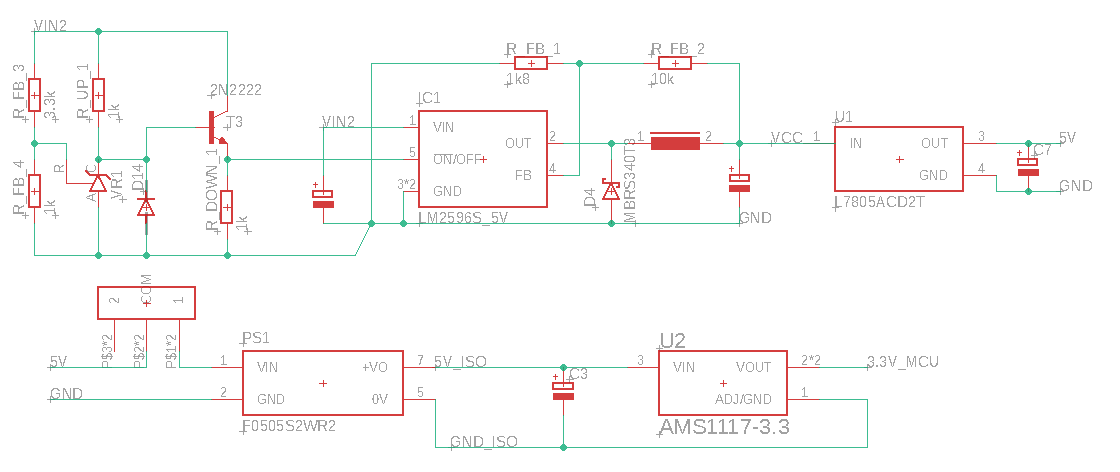
\includegraphics[width=\linewidth]{media/power_rail_schematic.png}}
        \caption{Power rail schematic.}
        \label{fig:power_rail_schematic}
    \end{figure}
    In this section, the input supply voltage, beside being used to power the connected load, is divided into two rails:
    \begin{enumerate}
        \item 5V rail.
        \item Isolated 5V rail.
    \end{enumerate}
    
    \pagebreak
    \subsection{5V rail}

    \subsubsection{Principle}
    \justify
    To supply power to the MOSFET driver circuit, latching circuit and the MCU, a 5V rail is needed. The following are methods of creating such constant voltage rail from the main power supply:

    \begin{table}[!h]
        \centering
        \begin{tabular}{|m{0.1\linewidth}|m{0.45\linewidth}|m{0.45\linewidth}|}
        
        \hline
        & Linear voltage regulator & Switching voltage regulator \\
        \hline
        Principle & 

        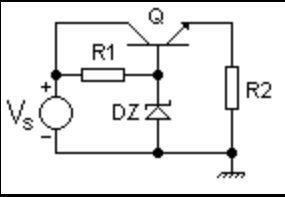
\includegraphics[width=0.3\textwidth]{media/series_regulator.png}
        \justify
        The above figure illustrates a simple circuit of a linear voltage regulator. In this circuit, assuming a constant load, the voltage drop across $R_2$ is kept constant by biasing the transistor $Q$ with zener diode $DZ$. &

        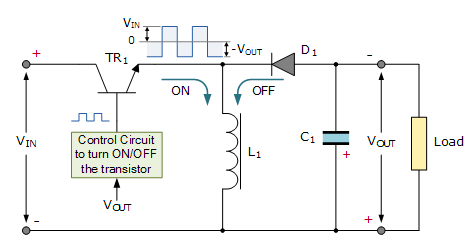
\includegraphics[width=0.45\textwidth]{media/inverting_switch_regulator.png}
        The above figure illustrates a simple switching voltage regulator. In this circuit, the close-open switching of the transistor stores and releases energy of the inductor which in turn charges the capacitor maintaining a constant voltage drop $V_{out}$ across the load. \\

        \hline
        Advantages & 

        \begin{itemize}
            \item Often comes as fixed output regulator.
            \item Requires very few external components. In case of fixed-output ones, only decouple capacitors are needed.
        \end{itemize} &
        
        \begin{itemize}
            \item Low power loss due to on/off switching of the transistor leading to less conduction loss.
            \item Can perform buck ($V_{out} < V_{in}$) and/or boost ($V_{out} > V_{in}$).
        \end{itemize} \\

        \hline
        Disadvantages & 

        \begin{itemize}
            \item High power loss: \newline $P_{loss} = P_{in} - P_{out} = (V_{in} - V_{load}) \cdot I_{e}$.
            \item Can only perform voltage step-down ($V_{out} < V_{in}$).
        \end{itemize} &
        
        \begin{itemize}
            \item High component count.
            \item Switching noise due to continuous charge and discharge of inductor.
            \item Lower load regulation capability, and are heavily dependent on the LC subcircuit. 
        \end{itemize}  \\

        \hline     
        \end{tabular}
        \caption{Comparison of linear and switching voltage regulator}
        \label{table:voltage_regulator_type}
    \end{table}

    \pagebreak
    \justify
    In this project, the MCU is the main source of current consumption. If a linear voltage regulator is used, then the power loss is:
    \begin{equation}
        \textbf{max}P_{loss} = (V_{in,max} - 5V) \cdot I_{MCU} = (30V - 5V) \cdot I_{MCU} = 5 \cdot (5V\cdot I_{MCU}) = 5P_{MCU}.
    \end{equation}  

    \justify
    The resulting efficiency is $\eta = 16.67\%$. To offset the disadvantages of the two type of voltage regulator, a hybrid where a step-down voltage regulator first reduce the input voltage to $V_{out,sw}=10V$, and a linear voltage regulator regulate $V_{out,sw}$ down to $5V$ (the desired voltage). With this setup, the followings are achieved:
    \begin{itemize}
        \item Lower power loss of $P_{loss} = (V_{out,sw} - 5V) \cdot I_{MCU} = (10V - 5V) \cdot I_{MCU}$.
        \item Switching noise and ripple of the switching regulator is reduced by the linear regulator. 
        \item $V_{out,sw}$ can be further reduced, as long as the switching regulator allows, to reduce the power loss even further.
    \end{itemize}

    \pagebreak
    \subsubsection{LM2596 and L7805xx}

    \justify
    LM2596 from Texas Instruments Inc. \cite{LM2596} is chosen for the construction of the switching regulator due to its few external component requirement. The IC has a built-in $3A$ switch, current-limit shutdown and TTL shutdown function on pin 5. By attaching a comparator circuit using a TL431 \cite{TL431} (See Figure \ref{fig:undervoltage_protection} to pin 5 of the LM2596, an undervoltage protection is applied, allowing only voltage above $V_{under\_thresh}$ to be step-down by the switching regulator. The calculation for $V_{under\_thresh}$ is as follow:

    \begin{equation}
        V_{under\_thresh} = (1+\dfrac{R_{FB\_3}}{R_{FB\_4}})\cdot V_{TL431\_ref} = (1+\dfrac{R_{FB\_3}}{R_{FB\_4}})\cdot 2.5V
    \end{equation}

    \begin{figure}[!h]
        \centerline{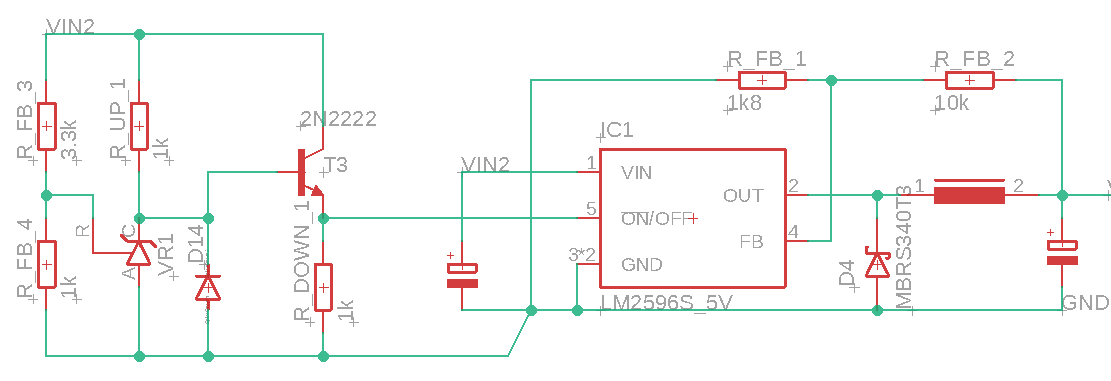
\includegraphics[width=\linewidth]{media/undervoltage_protection.png}}
        \caption{TL431-based undervoltage protection circuit.}
        \label{fig:undervoltage_protection}
    \end{figure}

    \justify
    The feedback for the switching regulator is done by $R_{FB\_2}$ and $R_{FB\_1}$. The values of the resistors follow the guide from the datasheet of the LM2596:

    \begin{equation}
        V_{out} = 1.23V(1 + \dfrac{R_{FB\_2}}{R_{FB\_1}})
    \end{equation}

    \justify
    L7805xx series from STMicroelectronics \cite{L78} is chosen for the linear voltage regulator due to its thermal and short-circuit protection. The IC also requires as little as two decoupling capacitors at the input and output stage.
    
    \pagebreak
    \subsection{Isolated 5V rail}
    \justify
    The needs of an isolated 5V rail are as follows:
    \begin{itemize}
        \item The MCU needs to be kept alive even if the input supply voltage malfunctions for diagnosis.
        \item The MCU needs to be connected to a laptop/PC to update the firmware. An isolated 5V rail prevents the potential of overvoltage damage dealt to external devices.
        \item The MCU is expensive and more difficult to replace than other components.
    \end{itemize}

    \justify
    Because the operation of the MCU is kept isolated from the input supply voltage, the user can choose to power it from the input supply or an external one.

    \justify
    To achieve this, the B0505S-2WR2 is chosen \cite{B0505}. The component supports $2W$ power, short-circuit protection and input voltage tolerance of $\pm 10 \%$.

\end{document}